% ============================================================
% chapters/07-risks.tex -- פרק 7: ניתוח סיכונים ותוכנית הפחתה
% Content only. All design comes from template.cls.
% Figure: figures/ch7-risk-matrix.pdf (code/make_figures.py)
% tab:risks and tab:mitigation MUST match RISKS in code/make_figures.py.
% ============================================================

\chapter{ניתוח סיכונים ותוכנית הפחתה}
\label{ch:risks}

כל סיכון במחקר מקבל שני ציונים, בסולם של 1 עד 5: \textbf{הסתברות} (\en{P}) – עד כמה סביר שיתממש, ו\textbf{חומרה} (\en{S}) – כמה נזק הוא יגרום אם יתממש. מכפלת שני הציונים היא \textbf{ציון הסיכון} (\en{$R = P \times S$}), וסיכון שציונו 12 ומעלה נחשב קריטי. טבלה~\ref{tab:risks} מזהה את הסיכונים המרכזיים ומכמתת אותם.

\begin{table}[htbp]
  \centering
  \caption{זיהוי הסיכונים וכימותם}
  \label{tab:risks}
  \small
  \begin{tabular}{cp{40mm}p{58mm}ccc}
    \toprule
    \textbf{מזהה} & \textbf{הסיכון} & \textbf{למה הוא עלול לקרות} & \textbf{\en{P}} & \textbf{\en{S}} & \textbf{\en{R}} \\
    \midrule
    \en{R1} & הטיית המקורות & רוב הטקסטים ששרדו נכתבו בידי אנשי כנסייה, שנוטים להציג את הכנסייה בתפקיד מרכזי (סעיף~\ref{sec:lit-method-issues}) & 4 & 4 & \textbf{16} \\
    \en{R2} & טעויות סיווג של המודל & מודלי שפה עלולים לטעות בלטינית וביוונית, ולעתים ״להמציא״ תשובות & 3 & 5 & \textbf{15} \\
    \en{R3} & חוסר נתונים & במערב של המאה החמישית יש מעט מספרים אמינים, ומקטעים שלמים עלולים להישאר ריקים & 4 & 3 & \textbf{12} \\
    \en{R4} & מדדים אנכרוניסטיים & מושגים מודרניים כמו ״יציבות״ או הפרדה בין ״כנסייה״ ל״מדינה״ אולי אינם מתאימים לתקופה \cite{obrien2026rise} & 3 & 4 & \textbf{12} \\
    \en{R5} & המומחה אינו זמין & התיקוף בחודש 5 נמצא על הנתיב הקריטי ותלוי באדם אחד & 2 & 4 & 8 \\
    \en{R6} & חריגה בעלות הטוקנים & ניתוח אלפי קטעים, ובמיוחד הרצות חוזרות, עלול לעלות יותר מהמתוכנן & 3 & 2 & 6 \\
    \bottomrule
  \end{tabular}
\end{table}

ארבעה מתוך ששת הסיכונים קריטיים לפני ההפחתה. לכל אחד מהם הוגדרו פעולת מנע, שמקטינה את הסיכוי שיתממש או את הנזק שלו, ותוכנית מגירה – מה עושים אם הוא בכל זאת מתממש (טבלה~\ref{tab:mitigation}).

\begin{table}[htbp]
  \centering
  \caption{פעולות מנע, תוכניות מגירה וציון שיורי}
  \label{tab:mitigation}
  \small
  \begin{tabular}{cp{56mm}p{48mm}c}
    \toprule
    \textbf{מזהה} & \textbf{פעולת מנע} & \textbf{תוכנית מגירה} & \textbf{\en{R} שיורי} \\
    \midrule
    \en{R1} & תיוג כל קטע לפי סוג המחבר; העדפת מקורות מסמכיים (חוקים, החלטות מועצות) על פני כרוניקות; ניתוח רגישות בלי כרוניקות שנכתבו בידי אנשי כנסייה & דיווח על כיוון ההטיה וניתוח נפרד לכל סוג מקור & 9 \\
    \en{R2} & תיקוף בשני סבבים; סוכן מבקר שמחפש טעויות; הרצה חוזרת לבדיקת עקביות (\en{REQ-AI-02}) & קטגוריות שנכשלות גם בסבב השני מקודדות ידנית בידי המומחה – מעבר חלקי לחלופה ב & 6 \\
    \en{R3} & טווח אי־ודאות לכל ערך, כמו במאגר \en{Seshat}; שימוש בממצאים ארכאולוגיים כמדדים עקיפים & איחוד מקטעים דלים למקטעים של 50 שנה & 4 \\
    \en{R4} & כמה מדדים נפרדים לכל מושג; התייעצות עם המומחה בבניית ספר ההגדרות; בדיקת הגדרות חלופיות & דיווח על כל מדד בנפרד, במקום מדד מסכם אחד & 4 \\
    \en{R5} & קביעת מועד התיקוף מראש; איתור מומחה שני כבר בתחילת המחקר & המומחה השני מבצע את התיקוף & 3 \\
    \en{R6} & תקרת תקציב; הערכת עלות מתוך הפיילוט; מודל זול יותר לשלבים פשוטים & סיווג של מדגם מייצג במקום של כל הקטעים & 4 \\
    \bottomrule
  \end{tabular}
\end{table}

איור~\ref{fig:risk-matrix} מציג את המעבר של כל סיכון במטריצה, מהמיקום שלו לפני ההפחתה (בעיגול אדום) אל המיקום שלו אחריה (בעיגול לבן).

\begin{figure}[htbp]
  \centering
  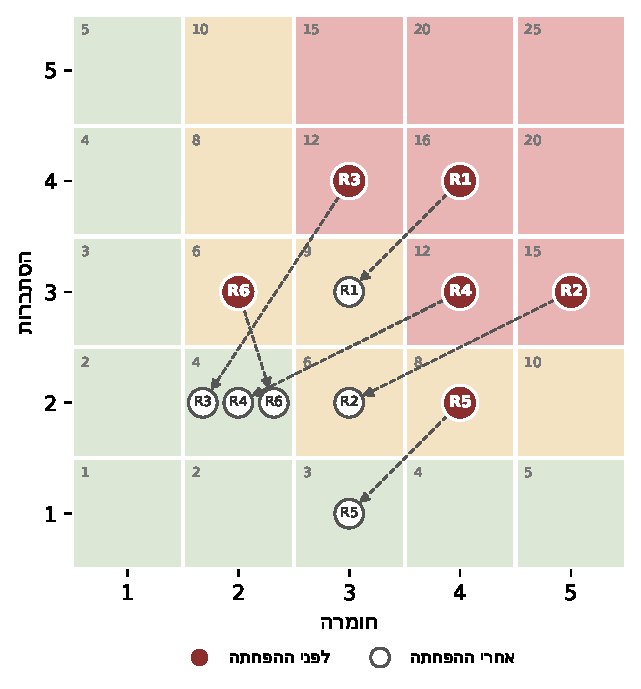
\includegraphics[width=0.62\textwidth]{figures/ch7-risk-matrix.pdf}
  \caption{מטריצת סיכונים: הסתברות מול חומרה, לפני ההפחתה ואחריה. האזור האדום הוא סיכון קריטי (\en{$R \geq 12$})}
  \label{fig:risk-matrix}
\end{figure}

\paragraph{מה נשאר.} אחרי ההפחתה אף סיכון אינו קריטי. הסיכון השיורי הגבוה ביותר הוא הטיית המקורות (\en{R1}), וזה לא מקרי: אי אפשר לבטל הטיה של מקורות שנכתבו לפני 1,500 שנה, אפשר רק למדוד אותה ולדווח עליה בשקיפות. לכן הדיון בתוצאות המחקר יכלול תמיד גם את השאלה ״מי כתב את המקור, ולמה״.
